\exercise
%
\begin{enumerate}

  \item Prove how an LCA query over an arbitrary tree can be turned into an RMQ
  query over an integer array.

  \item Describe the RMQ data structure that occupies space $O(n \log n)$ bits
  and answers queries $O(1)$ time.

  \item Show your transformation on the tree rooted in 1 and defined by the
  following edges $$\{ (1,2), (1,3), (1,4), (2,5), (2,6), (4,7) \},$$ and
  indicate how it is answered a query on the two leaves 5 and 7.

\end{enumerate}

\solution
%
\begin{enumerate}

  \item We can construct two arrays $E$ and $D$ of size $2e + 1 = O(n)$ where
  $e$ is the number of the edges of the tree, such that  $E$ contains the Euler
  Tour of the tree and $D$ the depth of each node in $E$. Solving a LCA problem
  over two leaves $L$ and $R$ of the tree is the same as solving the RMQ over
  the array $D[l, r]$, where $l$ and $r$ are, respectively, the positions of the
  leftmost and rightmost occurrence of $L$ and $R$ in $E$.

  \item Given the previous arrays $E$ and $D$, we build the matrix $M \in
  \mathbb{N}^{e \times \log_2 e} = O(n\log n)$ such that $$M_{i, j} =
  \operatorname*{argmin}_{k = j, \dots, j + 2^i - 1} D[k]\ .$$ For each range
  $[l, r]$, we can find the minimum of the sub-array $D[l, r]$ computing $$\min
  \left\{ D\big[M_{h, l}\big],\ D\big[M_{h, r - 2^h}\big] \right\}, \quad
  \text{with}\quad h = \lfloor \log_2 (r - l + 1)\rfloor\ .$$

  \item \autoref{fig:tree-depths-0} shows the graphical representation of the
  tree, while \autoref{tab:sparse-matrix} the values of $E$, $D$ and $M$ for
  this example. To compute the LCA(5, 7) we proceed as follows
  %
  \begin{enumerate}

    \item We first retrieve the position for the leftmost occurrence of 5 and
    the rightmost occurrence of 7 in the Euler Tour $E$, which are,
    respectively, $l = 3$ and $r = 11$.

    \item We evaluate $h = \lfloor\log_2 (r - l + 1) \rfloor = \lfloor\log_2 9
    \rfloor = 3$ and retrieve the positions of the RMQ in $D$ with $$M_{h, l} =
    M_{h, r - 2^h} = 7\ .$$ Since the cells of $M$ refer to the same position,
    we can state that LCA(5, 7) is $E[7] = 1$.

  \end{enumerate}
  %
  \begin{figure}[t]
    \centering
    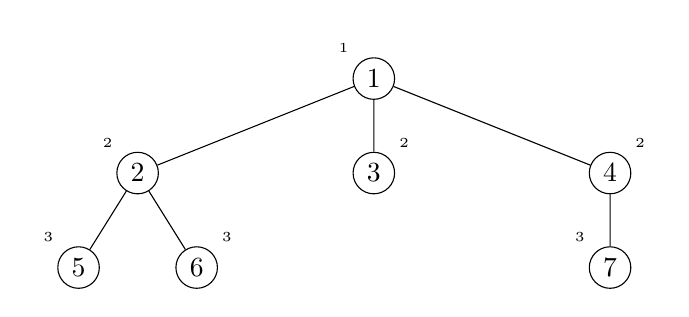
\begin{tikzpicture}[
      grow=down,
      every node/.style={draw, fill=white, inner sep=0, minimum size=15, circle},
      level 1/.style={sibling distance = 3cm, level distance = 1.2cm},
      level 2/.style={sibling distance = 1.5cm, level distance = 1.2cm}
    ]
    \node[label=135:{\tiny 1}] (1) {1}
    child {
      node[label=135:{\tiny 2}] (2) {2}
      child {
        node[label=135:{\tiny 3}] (5) {5}
        edge from parent[-]
      }
      child {
        node[label=45:{\tiny 3}] (6) {6}
        edge from parent[-]
      }
      edge from parent[-]
    }
    child {
      node[label=45:{\tiny 2}] (3) {3}
      edge from parent[-]
    }
    child {
      node[label=45:{\tiny 2}] (4) {4}
      child {
        node[label=135:{\tiny 3}] (7) {7}
        edge from parent[-]
      }
      edge from parent[-]
    };
    \end{tikzpicture}

    \caption{Graphical representation of the tree. The labels outside each node
    represents its depth.}

    \label{fig:tree-depths-0}
  \end{figure}
  %
  \begin{table}
    \centering
    \begin{tabular}{|r||c|c|c|c|c|c|c|c|c|c|c|c|c|}
      \multicolumn{1}{c}{} & \multicolumn{1}{c}{\tiny 1} &
      \multicolumn{1}{c}{\tiny 2} & \multicolumn{1}{c}{\tiny 3} &
      \multicolumn{1}{c}{\tiny 4} & \multicolumn{1}{c}{\tiny 5} &
      \multicolumn{1}{c}{\tiny 6} & \multicolumn{1}{c}{\tiny 7} &
      \multicolumn{1}{c}{\tiny 8} & \multicolumn{1}{c}{\tiny 9} &
      \multicolumn{1}{c}{\tiny 10} & \multicolumn{1}{c}{\tiny 11} &
      \multicolumn{1}{c}{\tiny 12} & \multicolumn{1}{c}{\tiny 13} \\
      \hline
      $E$ & 1 & 2 & 5 & 2 & 6 & 2 & 1 & 3 & 1 & 4 & 7 & 4 & 1 \\\hline
      $D$ & 1 & 2 & 3 & 2 & 3 & 2 & 1 & 2 & 1 & 2 & 3 & 2 & 1 \\\hline\hline
      $M_1$ & 1 & 2 & 4 & 4 & 6 & 7 & 7 & 9 & 9 & 10 & 12 & 13 & -- \\
      $M_2$ & 1 & 2 & 4 & 7 & 7 & 7 & 7 & 9 & 9 & 13 & -- & -- & -- \\
      $M_3$ & 1 & 7 & 7 & 7 & 7 & 7 & -- & -- & -- & -- & -- & -- & -- \\
      \hline
    \end{tabular}

    \caption{The values of $E$, $D$ and $M$.}
    \label{tab:sparse-matrix}
  \end{table}

\end{enumerate}
